\documentclass[tikz,border=10pt]{standalone}

\usepackage[utf8]{inputenc}
\usepackage[T1]{fontenc}
\usepackage{tikz}
\usetikzlibrary{positioning, arrows.meta}

\tikzset{
    box/.style = {
        rectangle,
        draw,
        rounded corners,
        minimum width=4cm,
        minimum height=0.9cm,
        align=center,
        font=\small
    },
    greenbox/.style = {box, fill=green!35},
    pinkbox/.style  = {box, fill=red!30},
    yellowbox/.style= {box, fill=yellow!50},
    graybox/.style  = {box, fill=gray!20},
    arrow/.style = {-{Latex[length=2mm]}, thick}
}

\begin{document}

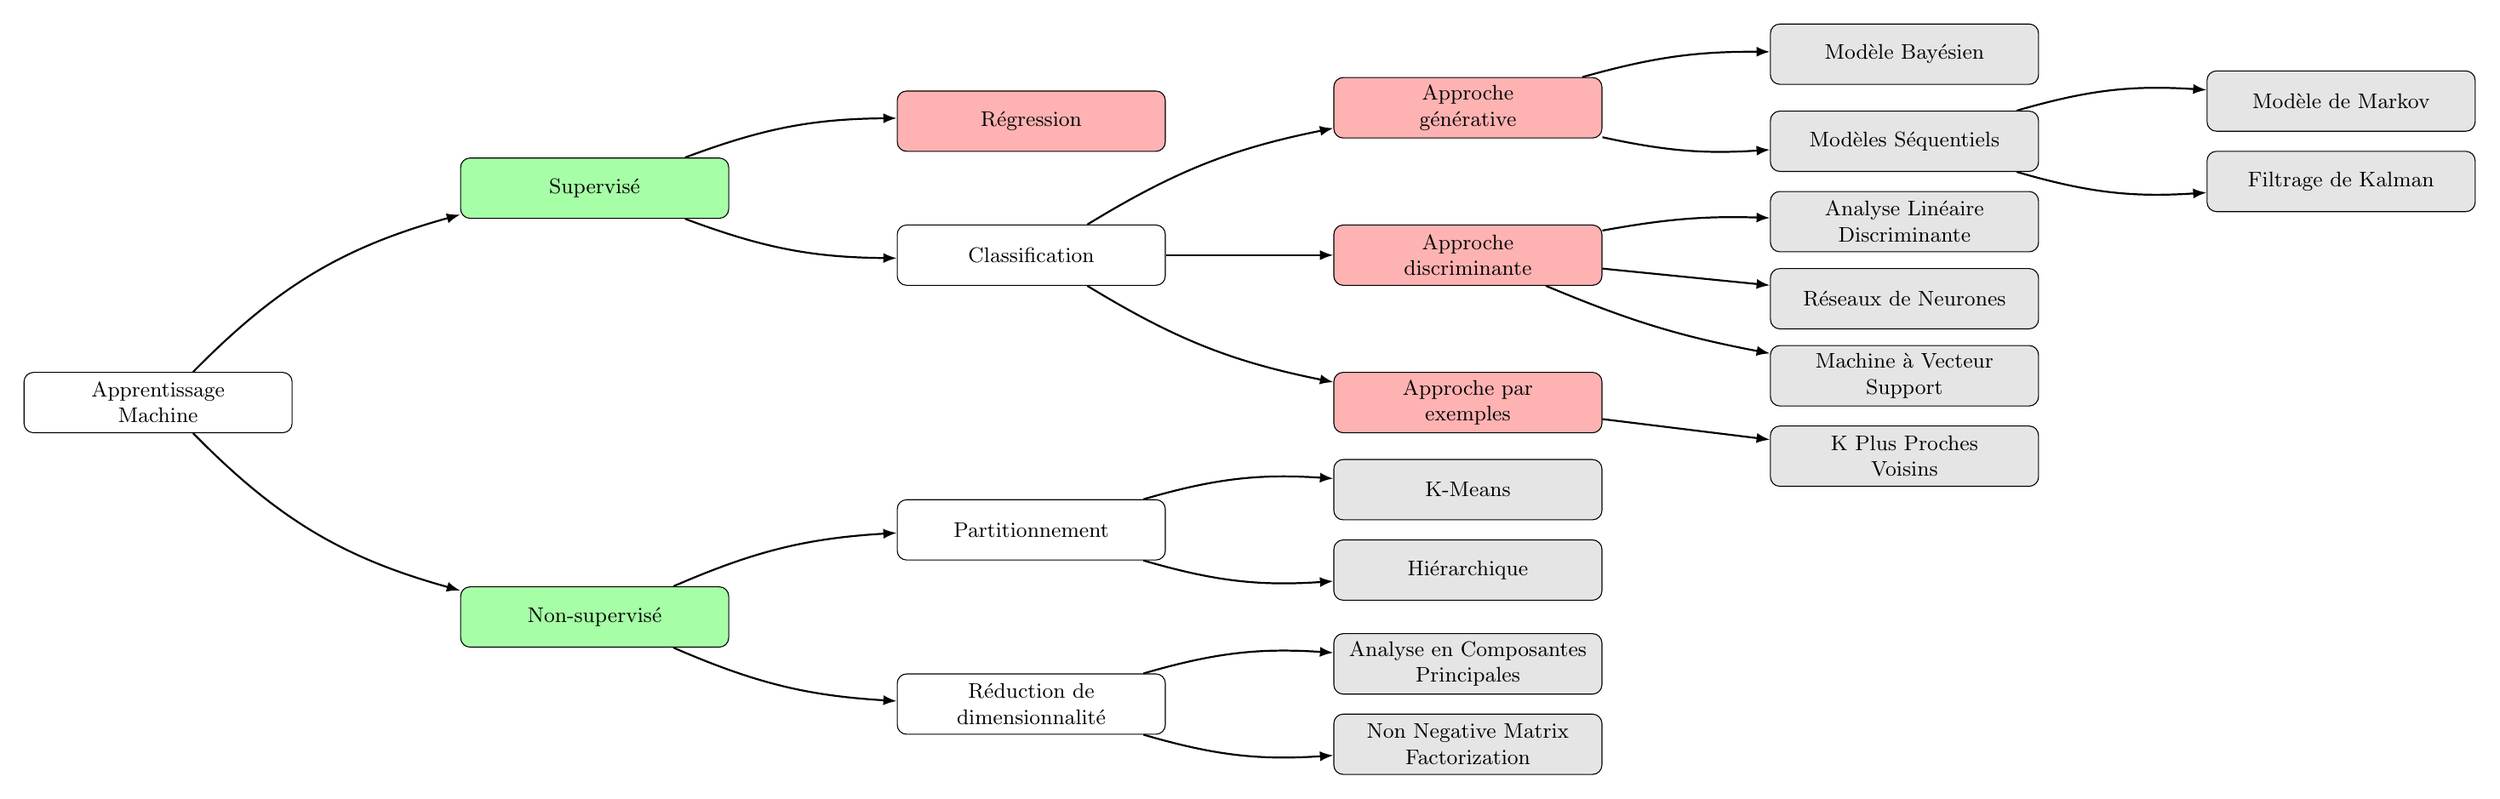
\begin{tikzpicture}[node distance=1.8cm and 2.5cm]

% Racine
\node[box] (ml) {Apprentissage\\Machine};

% Supervisé / Non-supervisé
\node[greenbox, right=of ml, yshift=3.2cm] (sup) {Supervisé};
\node[greenbox, right=of ml, yshift=-3.2cm] (unsup) {Non-supervisé};

\draw[arrow] (ml) to[bend left=15] (sup);
\draw[arrow] (ml) to[bend right=15] (unsup);

% --- SUPERVISÉ ---
\node[pinkbox, right=of sup, yshift=1.0cm] (reg) {Régression};
\node[box, right=of sup, yshift=-1.0cm] (classif) {Classification};


\draw[arrow] (sup) to[bend left=10] (reg);
\draw[arrow] (sup) to[bend right=10] (classif);


% Approches de classification
\node[pinkbox, right=of classif, yshift=2.2cm] (gen) {Approche\\générative};
\node[pinkbox, right=of classif] (disc) {Approche\\discriminante};
\node[pinkbox, right=of classif, yshift=-2.2cm] (ex) {Approche par\\exemples};

\draw[arrow] (classif) to[bend left=10] (gen);
\draw[arrow] (classif) -- (disc);
\draw[arrow] (classif) to[bend right=10] (ex);



% Générative → Bayes et Modèles séquentiels
\node[graybox, right=of gen, yshift=0.8cm] (bayes) {Modèle Bayésien};
\node[graybox, right=of gen, yshift=-0.5cm] (seq) {Modèles Séquentiels};

\draw[arrow] (gen) to[bend left=8] (bayes);
\draw[arrow] (gen) to[bend right=8] (seq);

\node[graybox, right=of seq, yshift=0.6cm] (hmm) {Modèle de Markov};
\node[graybox, right=of seq, yshift=-0.6cm] (kalman) {Filtrage de Kalman};

\draw[arrow] (seq) to[bend left=10] (hmm);
\draw[arrow] (seq) to[bend right=10] (kalman);

% Discriminante
\node[graybox, right=of disc, yshift=0.5cm] (lda) {Analyse Linéaire\\Discriminante};
\node[graybox, right=of disc, yshift=-0.65cm] (RN) {Réseaux de Neurones};
\node[graybox, right=of disc, yshift=-1.8cm] (svm) {Machine à Vecteur\\Support};

\draw[arrow] (disc) to[bend left=6] (lda);
\draw[arrow] (disc) -- (RN);
\draw[arrow] (disc) to[bend right=6] (svm);

% Par exemples
\node[graybox, right=of ex, yshift=-0.8cm] (knn) {K Plus Proches\\Voisins};
\draw[arrow] (ex) -- (knn);

% --- NON SUPERVISÉ ---
\node[box, right=of unsup, yshift=1.3cm] (part) {Partitionnement};
\node[box, right=of unsup, yshift=-1.3cm] (dimred) {Réduction de\\dimensionnalité};

\draw[arrow] (unsup) to[bend left=10] (part);
\draw[arrow] (unsup) to[bend right=10] (dimred);

\node[graybox, right=of part, yshift=0.6cm] (kmeans) {K-Means};
\node[graybox, right=of part, yshift=-0.6cm] (hier) {Hiérarchique};

\draw[arrow] (part) to[bend left=10] (kmeans);
\draw[arrow] (part) to[bend right=10] (hier);

\node[graybox, right=of dimred, yshift=0.6cm] (pca) {Analyse en Composantes\\Principales};
\node[graybox, right=of dimred, yshift=-0.6cm] (nmf) {Non Negative Matrix\\Factorization};

\draw[arrow] (dimred) to[bend left=10] (pca);
\draw[arrow] (dimred) to[bend right=10] (nmf);

\end{tikzpicture}

\end{document}
